\section{Parte 04 – Instalacion de Oracle Data 12C} 
\begin{enumerate}[1.]
	      
	\item Ingresamos nuevamente a Administraci\'on de equipos y seleccionamos  la opci\'on de usuarios y grupos locales.\\
	\begin{center}
	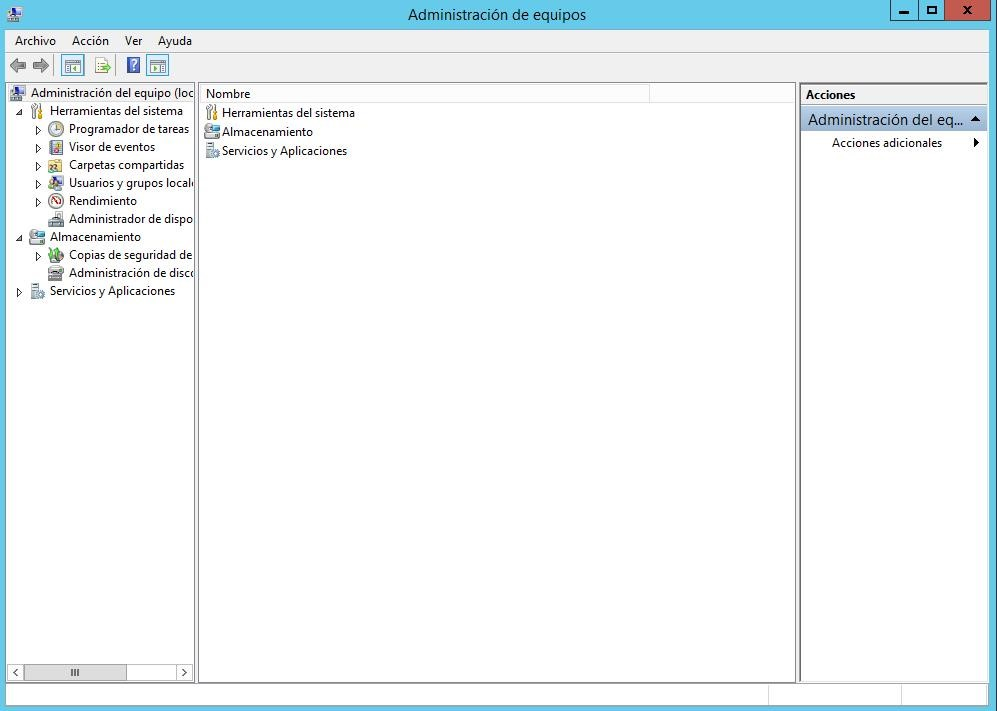
\includegraphics[width=10cm]{./Imagenes/jhordy1} 
	\end{center}
	\hfill \break	
	\hfill \break
	\hfill \break
	\hfill \break
	\begin{center}
	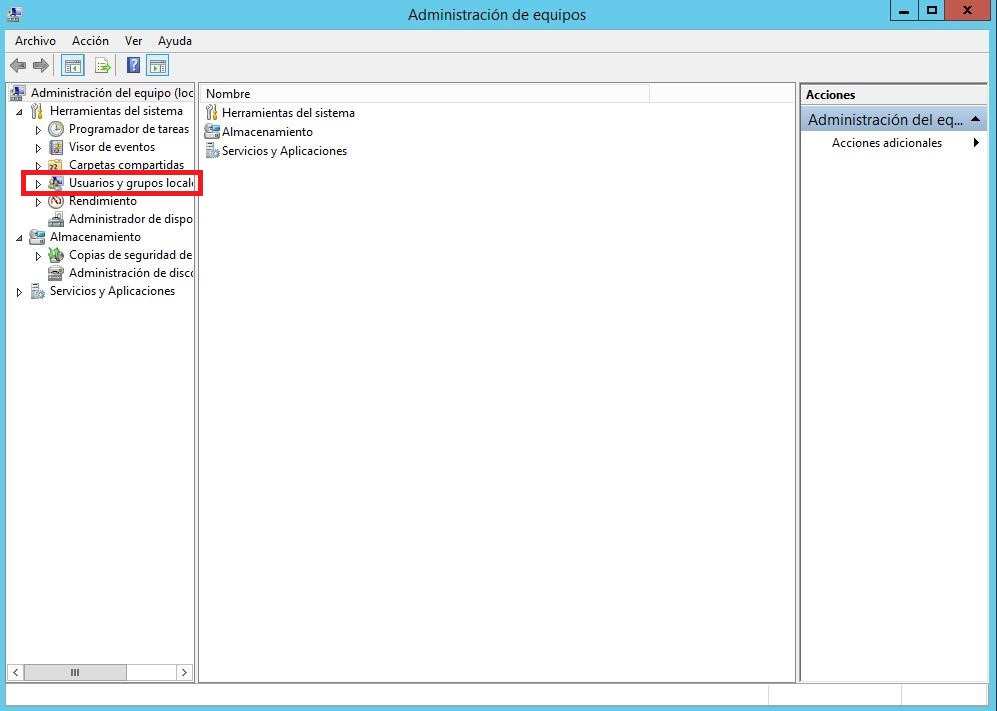
\includegraphics[width=10cm]{./Imagenes/jhordy11} 
	\end{center}
	\hfill \break
	\hfill \break
	\hfill \break
	\hfill \break
	\item Ingresamos a la carpeta de Usuarios y nos vamos a la opci\'on de equipos ORACLE.\\
	\begin{center}
	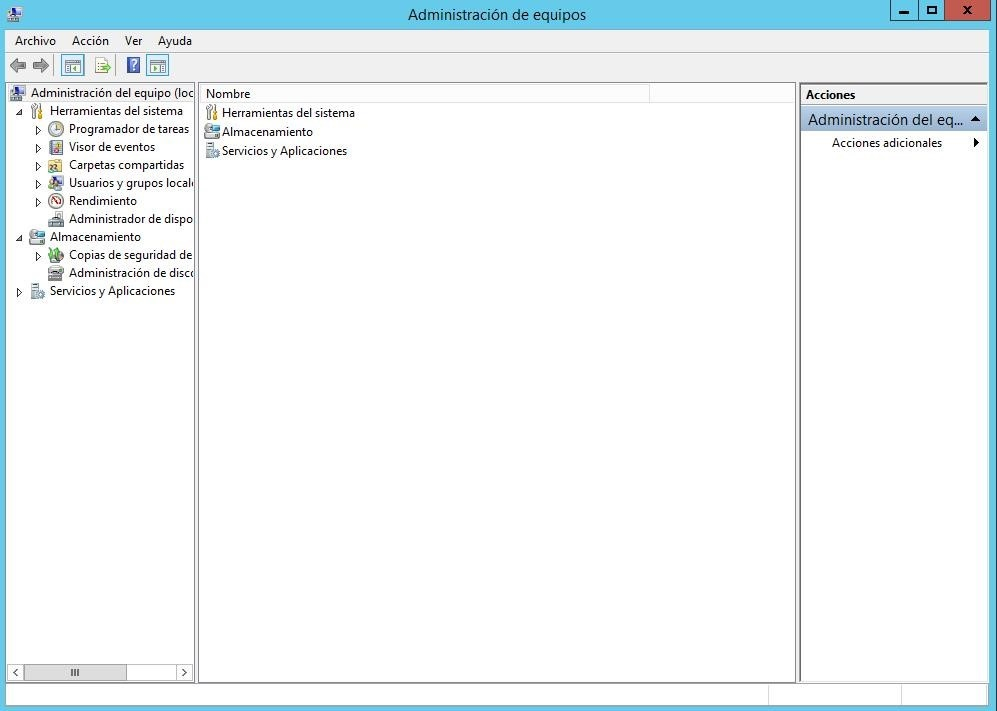
\includegraphics[width=10cm]{./Imagenes/jhordy2} 
	\end{center}
	\hfill \break
	\hfill \break
	\hfill \break
	\hfill \break
	\item Una vez realizado eso reiniciamos el servidor y al usuario ORACLE.\\
	\begin{center}
	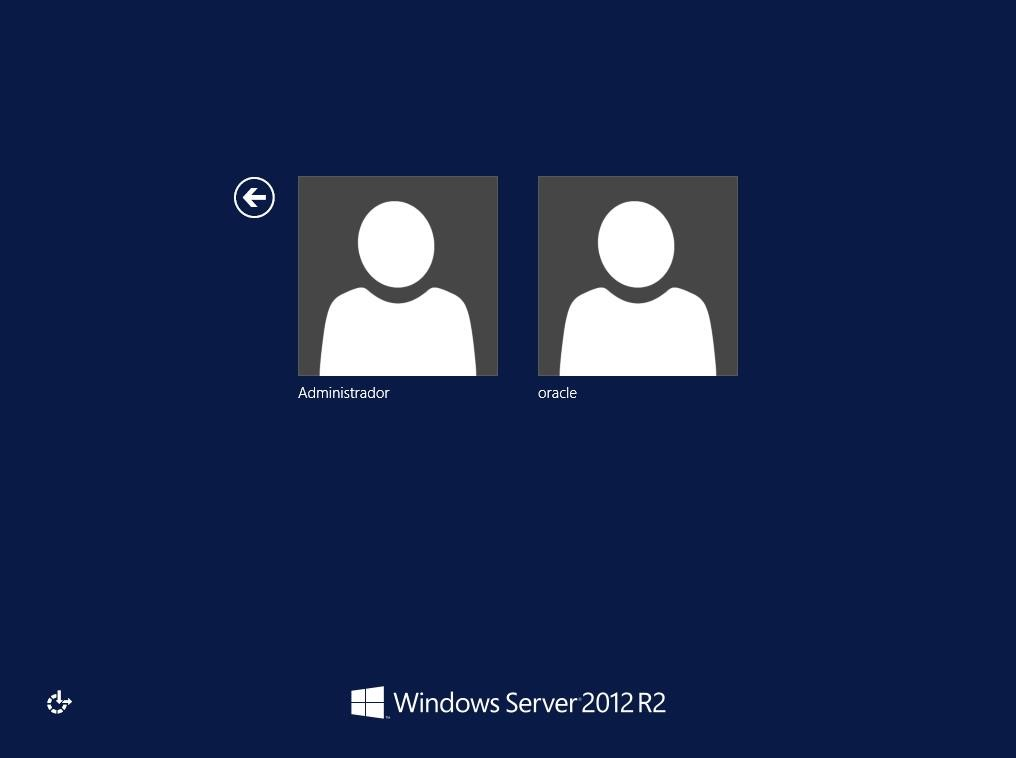
\includegraphics[width=10cm]{./Imagenes/jhordy3} 
	\end{center}
	\hfill \break
	\hfill \break
	\hfill \break
	\hfill \break
	\item Colocamos la clave de administrador que es  "UPT2018".\\
	\begin{center}
	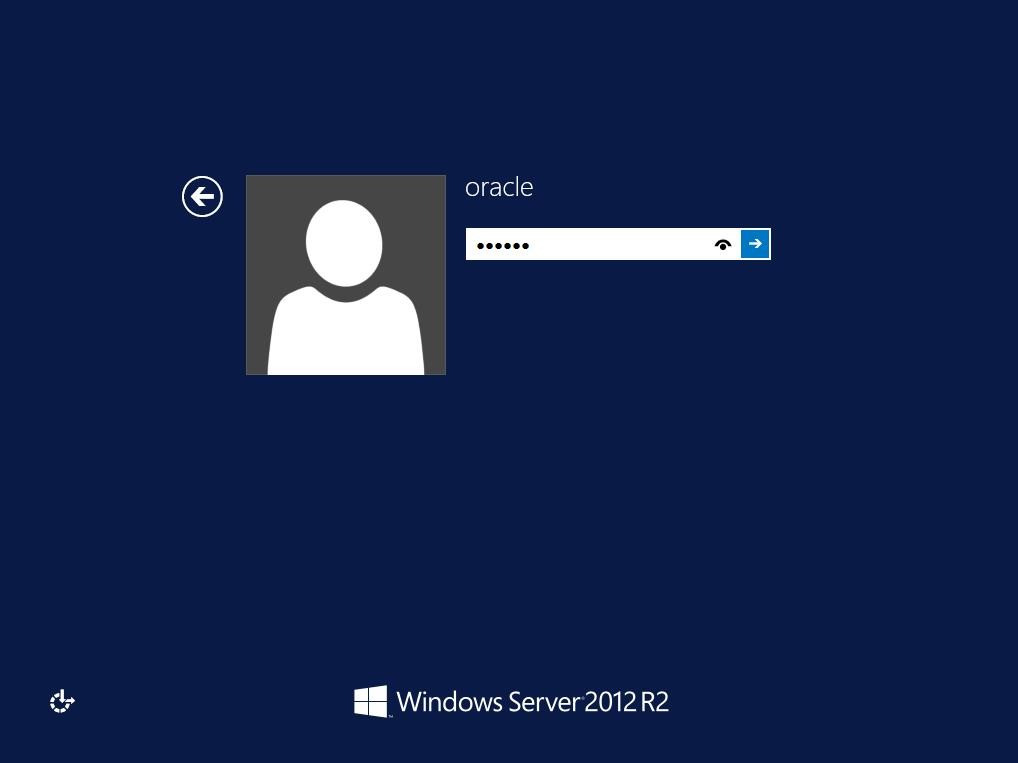
\includegraphics[width=10cm]{./Imagenes/jhordy4} 
	\end{center}
	\hfill \break
	\hfill \break
	\hfill \break
	\hfill \break
	\item Empezaremos la instalaci\'on de la base de datos ORACLE seleccionando el archivo ejecutable "setup" a setup.\\
	\begin{center}
	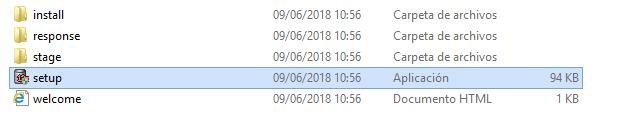
\includegraphics[width=10cm]{./Imagenes/jhordy5} 
	\end{center}
	\hfill \break
	\hfill \break
	\hfill \break
	\hfill \break
	\hfill \break
	\item Instalamos como el usuario administrador, colocando la clave de usuario.\\
	\begin{center}
	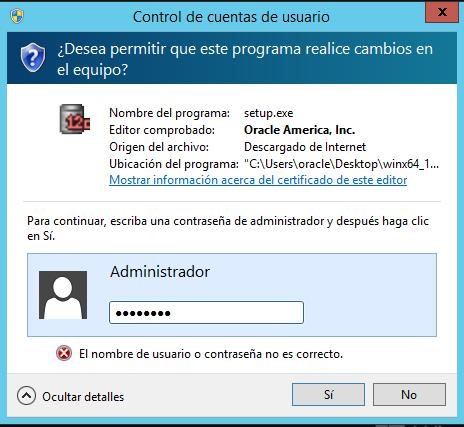
\includegraphics[width=10cm]{./Imagenes/jhordy6} 
	\end{center}
	\hfill \break
	\hfill \break
	\hfill \break
	\hfill \break
	\item Procede autom\'aticamente la instalaci\'on del ORACLE\\
	\begin{center}
	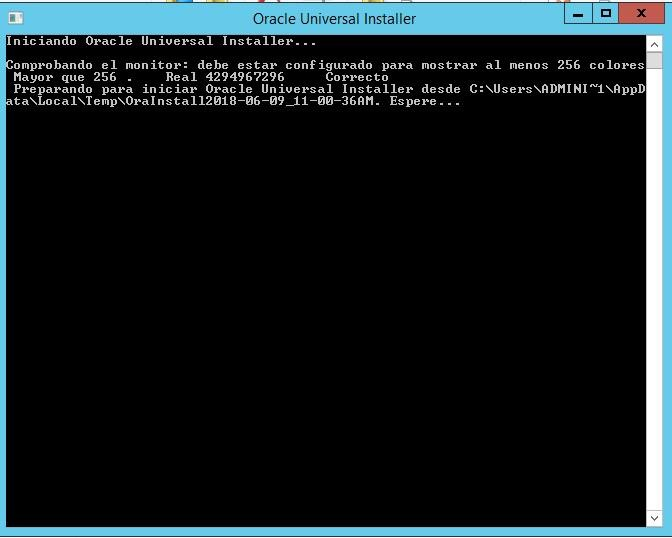
\includegraphics[width=10cm]{./Imagenes/jhordy7} 
	\end{center}
	\hfill \break
	\hfill \break
	\hfill \break
	\hfill \break
	\hfill \break
	\hfill \break
	\hfill \break
	\hfill \break
	\hfill \break
	\item Nos aparece la pantalla de configuraci\'on.\\
	\begin{center}
	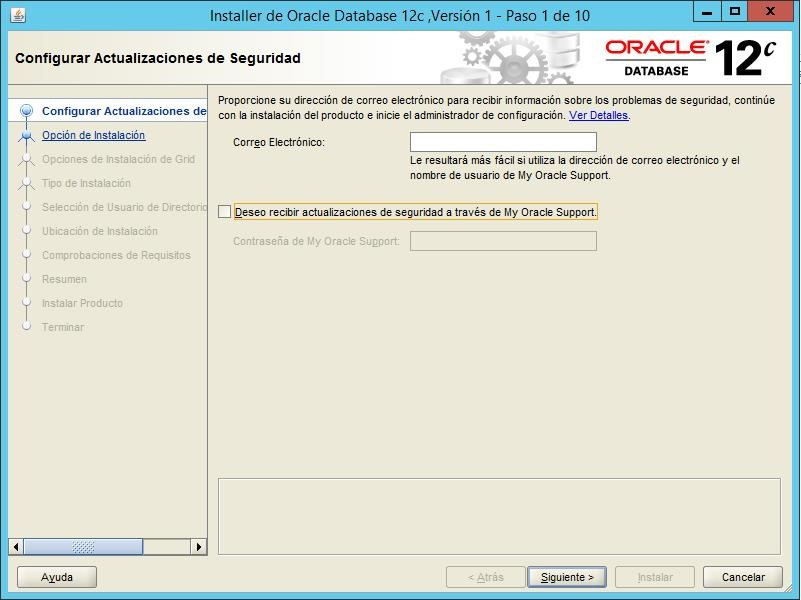
\includegraphics[width=10cm]{./Imagenes/jhordy8} 
	\end{center}

           \item  Nos saldra un aviso ingresar su correo  electronico , colocaremos si.
 	\begin{center}
	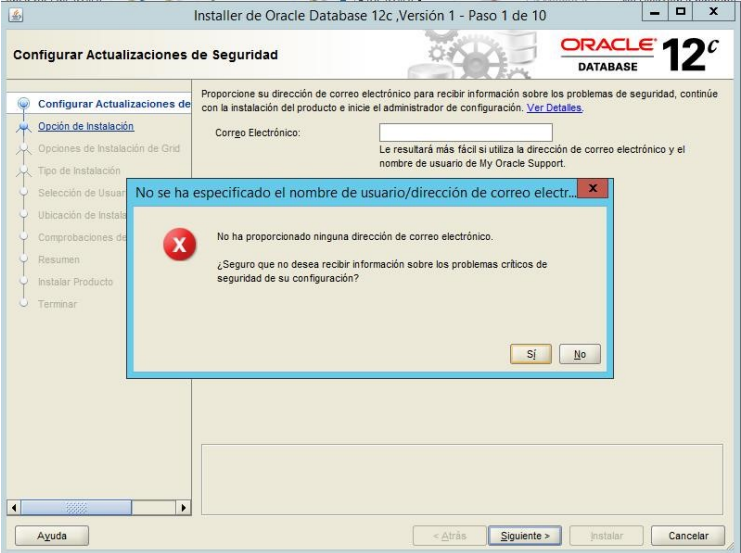
\includegraphics[width=10cm]{./Imagenes/bran1} 
	\end{center}
           \item Elegimos la opcion de Crear y configurar Base de Datos
 	\begin{center}
	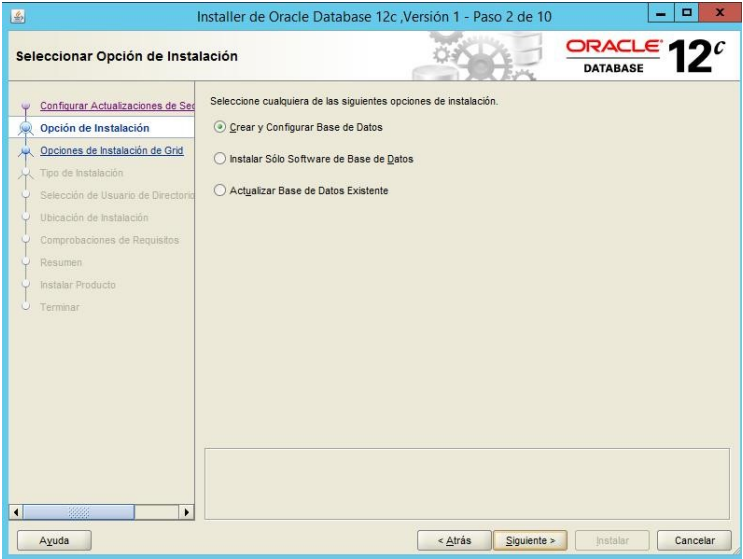
\includegraphics[width=10cm]{./Imagenes/bran2} 
	\end{center}
          \item Nos aparecera 2 opciones, que clase de sistema queremos instalar escogemos la opcion Clase escritorio.
 	\begin{center}
	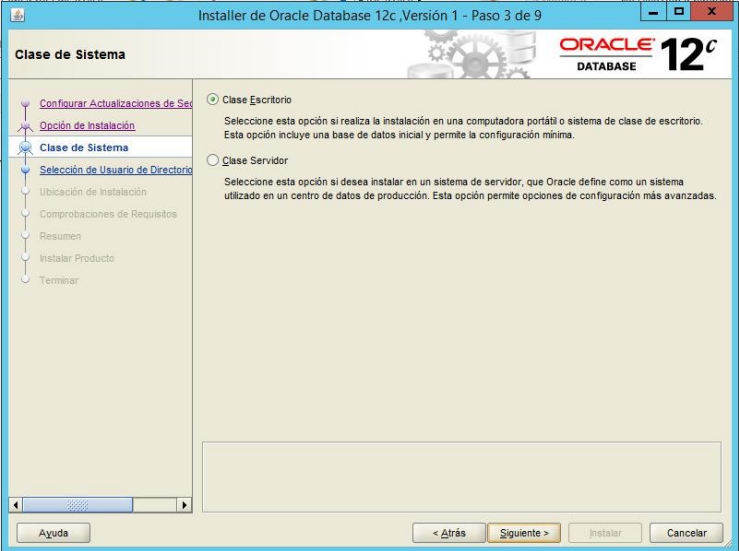
\includegraphics[width=10cm]{./Imagenes/bran3} 
           \end{center}
	\hfill \break
	\hfill \break
	\hfill \break
	\hfill \break
	\hfill \break
	\hfill \break
	\hfill \break
	\hfill \break
	\hfill \break
	\hfill \break
	\hfill \break
	\hfill \break
          \item Luego ingresamos con nuestro usuario y contrase\~na, seleccion
 	\begin{center}
	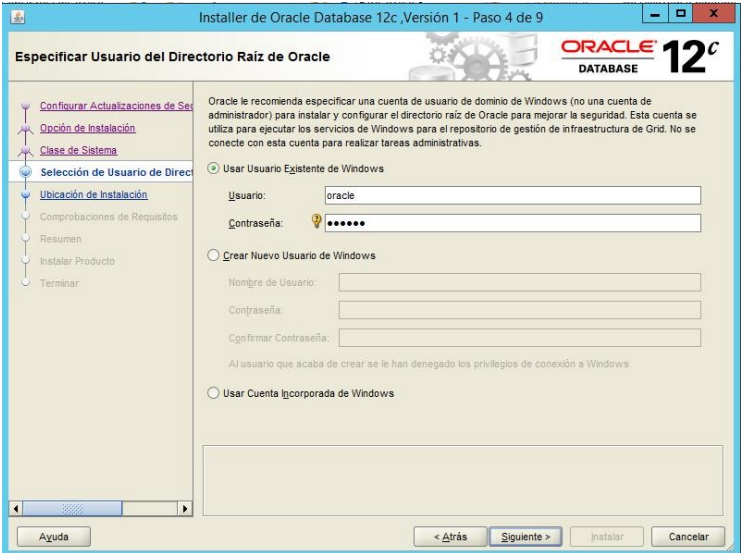
\includegraphics[width=10cm]{./Imagenes/bran4} 
	\end{center}
	\item Realizamos las opciones de configuracion, llenando los datos especificos.
 	\begin{center}
	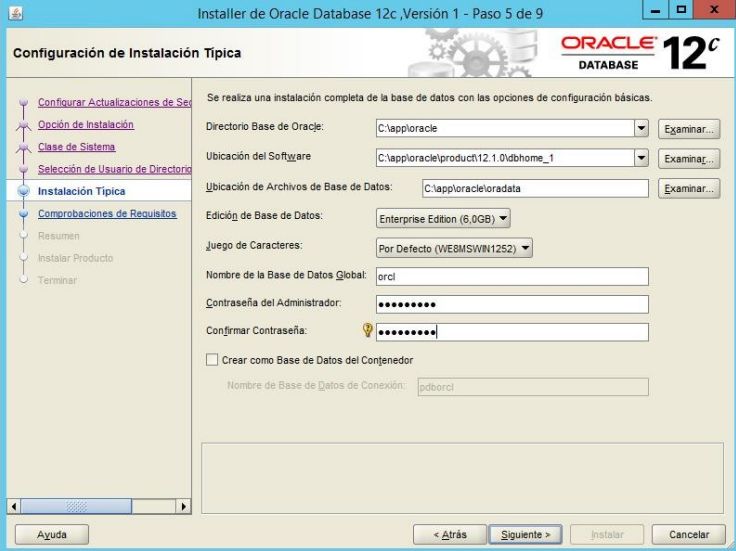
\includegraphics[width=10cm]{./Imagenes/bran5} 
	\end{center}
	\hfill \break
	\hfill \break
	\hfill \break
	\hfill \break
	\hfill \break
	\hfill \break
	\hfill \break
	\hfill \break
	\hfill \break
	\hfill \break
	\hfill \break
	\hfill \break
          \item Verificacion de datos y comprobaciones
 	\begin{center}
	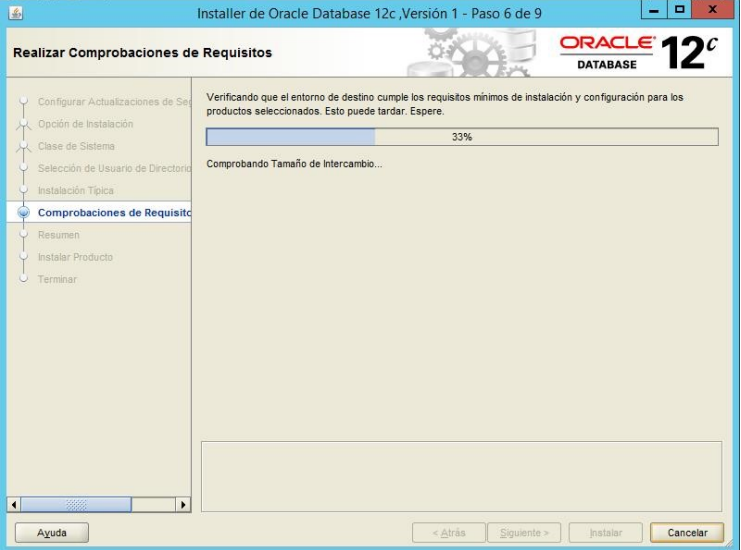
\includegraphics[width=10cm]{./Imagenes/bran6} 
	\end{center}
          \item Luego nos muestra una pantalla con el resumen de instalacion
 	\begin{center}
	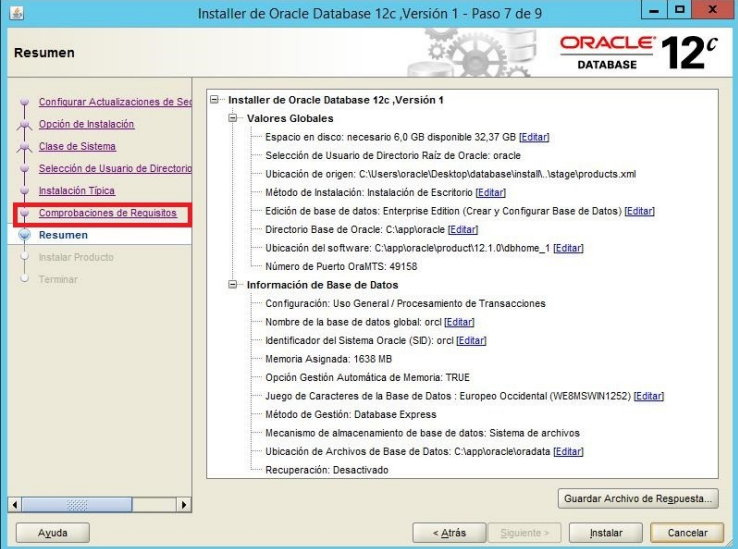
\includegraphics[width=10cm]{./Imagenes/bran7} 
	\end{center}
	\hfill \break
	\hfill \break
	\hfill \break
	\hfill \break
	\hfill \break
	\hfill \break
	\hfill \break
	\hfill \break
	\hfill \break
	\hfill \break
	\hfill \break
	\hfill \break
           \item Seguidamente muestra una pantalla de comprobacion nuestros requisitos y colocamos siguientes.
 	\begin{center}
	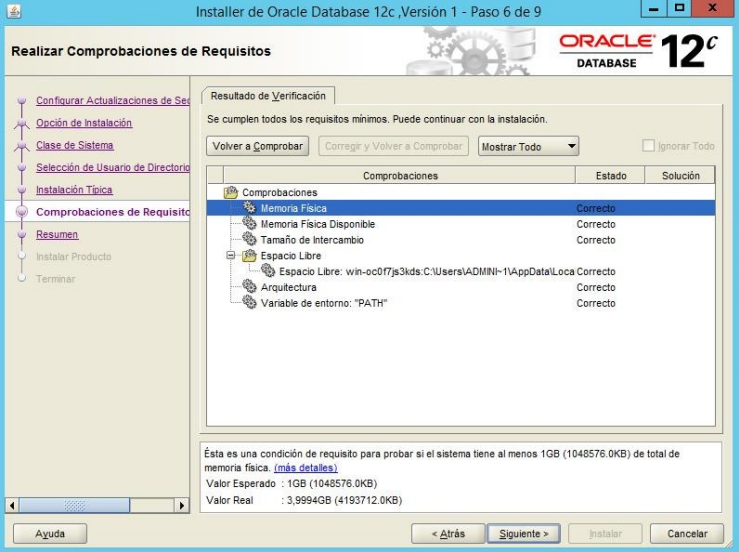
\includegraphics[width=10cm]{./Imagenes/bran8} 
	\end{center}
	
\end{enumerate} 
